\documentclass[]{vvsu}

\vvsuyear{2025}

%%%%%%%%%%%%%%%%%%%

\usepackage{graphicx} % для изображений
\usepackage{tabularray} % для таблиц
\usepackage{siunitx} % для обозначений (процент, градус)
\usepackage{listings} % для листингов кода

% Список путей, где будут искаться изображения и файлы
\graphicspath{{images/}}

% Файл со списком источников (не используется)
% \addbibresource{./references.bib}

% Автор документа
\author{А.И. Студент}

% Настройка стилей для листингов кода
\setmonofont{Consolas}

\makeatletter

\newcommand\language@yaml{yaml}
\expandafter\expandafter\expandafter\lstdefinelanguage
\expandafter{\language@yaml}
{
  keywords={true,false,null,y,n},
  keywordstyle=\color{darkgray},
  basicstyle=\setmainfont{Consolas}\fontsize{8}{8}\linespread{1}\selectfont,
  sensitive=false,
  comment=[l]{\#},
  morecomment=[s]{/*}{*/},
  commentstyle=\color{purple},
  stringstyle=\color{blue},
  moredelim=[l][\color{orange}]{\&},
  moredelim=[l][\color{magenta}]{*},
  moredelim=**[il][\color{red}{:}\color{blue}]{:},
  morestring=[b]',
  morestring=[b]",
  literate =    {---}{{\ProcessThreeDashes}}3
                {>}{{\textcolor{red}\textgreater}}1
                {|}{{\textcolor{red}\textbar}}1
                {\ -\ }{{\ -\ }}3,
}
\lst@AddToHook{EveryLine}{\ifx\lst@language\language@yaml\color{black}\fi}
\makeatother

\lstdefinelanguage{json}{
    basicstyle=\fontsize{8}{8}\linespread{1}\selectfont\ttfamily,
    sensitive=false,
    stringstyle=\color{blue},
    string=[s]{":\ "}{"},
    literate=
        *{0}{{{\color{red}0}}}{1}
         {1}{{{\color{red}1}}}{1}
         {2}{{{\color{red}2}}}{1}
         {3}{{{\color{red}3}}}{1}
         {4}{{{\color{red}4}}}{1}
         {5}{{{\color{red}5}}}{1}
         {6}{{{\color{red}6}}}{1}
         {7}{{{\color{red}7}}}{1}
         {8}{{{\color{red}8}}}{1}
         {9}{{{\color{red}9}}}{1}
}

\definecolor{codegray}{rgb}{0.5,0.5,0.5}
\definecolor{backcolour}{rgb}{0.95,0.95,0.92}
\lstdefinestyle{codestylelst}{
    backgroundcolor=\color{backcolour},
    numberstyle=\color{codegray}\ttfamily,
    breakatwhitespace=false,
    breaklines=true,
    captionpos=b,
    keepspaces=true,
    numbers=left,
    numbersep=5pt,
    showspaces=false,
    showstringspaces=false,
    showtabs=false,
    tabsize=2
}
\lstset{style=codestylelst}


%%%%%%%%%%%%%%%%%%%

\begin{document}

% Шапка
\vvsuhead{\linespread{1}\selectfont{}МИНОБРНАУКИ РОССИИ\\
\vspace{10pt}Федеральное государственное бюджетное образовательное учреждение\\
высшего образования\\
\fontsize{13}{13}\selectfont{}<<ВЛАДИВОСТОКСКИЙ ГОСУДАРСТВЕННЫЙ УНИВЕРСИТЕТ>>\\
(ФГБОУ ВО <<ВВГУ>>)\\
\vspace{10pt}\fontsize{12}{12}\selectfont{}ИНСТИТУТ ИНФОРМАЦИОННЫХ ТЕХНОЛОГИЙ И АНАЛИЗА ДАННЫХ\\
КАФЕДРА ИНФОРМАЦИОННЫХ ТЕХНОЛОГИЙ И СИСТЕМ}

% Название отчета
\title{Отчет\\по лабораторной работе №1}
\subtitle{по дисциплине\\<<Информатика и программирование>>}

% Участники работы
\member{Студент\\ гр. GGG-NN-LL}{А.И. Студент}
\member{Ассистент\\ преподавателя}{М.В. Водяницкий}

% Вывод титульника
\maketitle

% Задание
% Задание
\begin{addition}{Задание}
  Выполнить задания на Python и оформить отчет по стандартам ВВГУ.

  \textit{\textbf{Задание 1.}}  
  Объявить четыре переменные с любыми значениями для каждого из основных типов данных (int, float, str, bool).

  \textit{\textbf{Задание 2.}}  
  Объявить две переменные: одну для вашего имени, другую для вашего возраста. Затем вывести значения переменных в консоль.

  \textit{\textbf{Задание 3.}}  
  Объявить три переменные: одну со значением 342, вторую со значением 56.2 и третью со значением '43'.  
  Найти сумму всех трех чисел и результат записать в новую переменную. Вывести значение новой переменной в консоль.

  \textit{\textbf{Задание 4.}}  
  Объявить переменные a и b со значениями 3 и 8.  
  Вычислить значение уравнения $(a + 4b)(a - 3b) + a ^ 2$ и вывести результат в консоль.

  \textit{\textbf{Задание 5.}}  
  Написать программу для вычисления площади и периметра прямоугольника.  
  Данные сторон прямоугольника должны запрашиваться у пользователя и вводиться с консоли.  
  Результат работы программы вывести в консоль.

  \textit{\textbf{Задание 6.}}  
  Вывести в консоль букву w, составленную из символов *, расположенных в три строки.

  Пример:
  \begin{verbatim}
      *   *   *
       * * * *
        *   *\end{verbatim}

  \textit{\textbf{Задание 7.}}  
  Создать две переменные с любыми именами и любыми числовыми значениями.  
  Вывести в консоль результат выполнения всех арифметических операторов (7 операторов) и операторов сравнения (6 операторов).

  \textit{\textbf{Задание 8.}}  
  Создать две переменные: одну для вашего имени, другую для вашего возраста.  
  С помощью f-строки вывести в консоль строку вида:  
  Меня зовут <ваше имя>, мне <ваш возраст> лет.

  \textit{\textbf{Задание 9.}}  
  Разбить предложение Съешь еще этих мягких французских булок, да выпей чаю 
  на несколько переменных, содержащих по одному-два слова.  
  Затем с помощью конкатенации строк необходимо собрать предложение вновь и вывести в консоль (не забывайте про пробелы).

  \textit{\textbf{Задание 10.}}  
  Составить предложение, состоящее из строки <<Нет! Да!>>, которая повторяется 4 раза (используйте умножение строк).

  \textit{\textbf{Задание 11.}}  
  Запросить на ввод с консоли три числа, разделенных запятой,  
  и записать их в три отдельные переменные.  
  Затем первое и третье число сложить и результат целочисленно разделить на второе число.  
  Конечный результат вывести в консоль в виде строки:  
  Результат вычисления: <результат>.

  \textit{\textbf{Задание 12.}}  
  Запросить на ввод с консоли слово, содержащее не менее 10 символов.  
  С помощью срезов вывести:
  \begin{vvsu_list}
    \item первые 4 символа;
    \item последние 2 символа;
    \item символы от 4 до 8;
    \item перевернутое слово.
  \end{vvsu_list}
\end{addition}

% Содержание
\toc

% Глава - Выполнение работы
\section{Выполнение работы}

% Подглава - Задание 1
\subsection{Задание 1}

В данном задании были созданы четыре переменные, каждая из которых относится к одному из основных типов данных: целые числа, числа с плавающей точкой, строки и логические значения. После объявления переменные были выведены на экран с помощью функции print(). На рисунке \ref{fig:code_task_1} представлен код полученной программы.

\begin{vvsu_figure}{Листинг программы для задания 1}{fig:code_task_1}
  \begin{minipage}{.75\textwidth}
    \lstinputlisting[language=Python,basicstyle=\fontsize{10}{10}\linespread{1}\selectfont\ttfamily]{code/task1.py}
  \end{minipage}
\end{vvsu_figure}

Пояснение работы программы:
\begin{vvsu_list}
  \item переменная a имеет тип int и хранит целое число;
  \item переменная b имеет тип float и хранит дробное число;
  \item переменная c содержит строковое значение, заключенное в кавычки;
  \item переменная d является логической и может принимать значения True или False.
\end{vvsu_list}

После выполнения программы в консоль последовательно выводятся значения всех четырех переменных.

% Подглава - Задание 2
\subsection{Задание 2}

В данном задании были созданы две переменные: одна хранит имя пользователя, другая -- его возраст. После присвоения значений обе переменные выводятся в консоль с помощью функции print(). На рисунке \ref{fig:code_task_2} представлен код программы.

\begin{vvsu_figure}{Листинг программы для задания 2}{fig:code_task_2}
  \begin{minipage}{.75\textwidth}
    \lstinputlisting[language=Python,basicstyle=\fontsize{10}{10}\linespread{1}\selectfont\ttfamily]{code/task2.py}
  \end{minipage}
\end{vvsu_figure}

Пояснение работы программы:
\begin{vvsu_list}
  \item Переменная name содержит строковое значение -- имя пользователя.
  \item Переменная age содержит целое значение -- возраст пользователя.
  \item Функция print() выводит оба значения через пробел в одной строке.
\end{vvsu_list}

% После выполнения программы в консоли отображается имя и возраст пользователя.

% Подглава - Задание 3ыы
\subsection{Задание 3}

В этом задании необходимо было объявить три переменные: две числовые и одну строковую, содержащую число. Затем требовалось найти сумму всех трёх чисел и вывести результат в консоль. На рисунке \ref{fig:code_task_3} представлен код программы.

\begin{vvsu_figure}{Листинг программы для задания 3}{fig:code_task_3}
  \begin{minipage}{.75\textwidth}
    \lstinputlisting[language=Python,basicstyle=\fontsize{10}{10}\linespread{1}\selectfont\ttfamily]{code/task3.py}
  \end{minipage}
\end{vvsu_figure}

Пояснение работы программы:
\begin{vvsu_list}
  \item Переменная a хранит целое число 342.
  \item Переменная b хранит дробное число 56.2.
  \item Переменная c содержит строку <<43>>, которая преобразуется в число \linebreak функцией int().
  \item Сумма трёх чисел сохраняется в переменной result и выводится функцией print().
\end{vvsu_list}

В результате выполнения программа выводит сумму трёх значений, приведённых к числовому типу.

% Подглава - Задание 4
\subsection{Задание 4}

В задании необходимо было вычислить значение выражения $(a + 4b)(a - 3b) + a^2$ для заданных переменных. На рисунке \ref{fig:code_task_4} представлен код решения.

\begin{vvsu_figure}{Листинг программы для задания 4}{fig:code_task_4}
  \begin{minipage}{.75\textwidth}
    \lstinputlisting[language=Python,basicstyle=\fontsize{10}{10}\linespread{1}\selectfont\ttfamily]{code/task4.py}
  \end{minipage}
\end{vvsu_figure}

Пояснение работы программы:
\begin{vvsu_list}
  \item Переменным a и b присвоены значения 3 и 8.
  \item Выражение вычисляется в соответствии с математическими правилами приоритета операций.
  \item Оператор ** используется для возведения числа a в квадрат.
  \item Результат сохраняется в переменной result и выводится в консоль.
\end{vvsu_list}

После выполнения программы в консоли отображается вычисленное\linebreak значение выражения.

% Подглава - Задание 5
\subsection{Задание 5}

Цель задания -- реализовать программу для вычисления площади и периметра прямоугольника, стороны которого вводятся пользователем с консоли. На рисунке \ref{fig:code_task_5} представлен код программы.

\begin{vvsu_figure}{Листинг программы для задания 5}{fig:code_task_5}
  \begin{minipage}{.75\textwidth}
    \lstinputlisting[language=Python,basicstyle=\fontsize{10}{10}\linespread{1}\selectfont\ttfamily]{code/task5.py}
  \end{minipage}
\end{vvsu_figure}

Пояснение работы программы:
\begin{vvsu_list}
  \item С помощью функции input() запрашиваются длины сторон прямоугольника, которые преобразуются в тип float.
  \item Переменная area вычисляется как произведение сторон прямоугольника.
  \item Переменная perimeter вычисляется по формуле $2 * (width + height)$.
  \item Оба результата выводятся на экран при помощи функции print().
\end{vvsu_list}

После запуска программы пользователь вводит значения сторон и получает площадь и периметр прямоугольника.

% Подглава - Задание 6
\subsection{Задание 6}

В данном задании необходимо было вывести в консоль символическую (ASCII-art) букву w, составленную из символов *, расположенных в три строки.  
Для реализации задачи использовались последовательные вызовы функции print(), каждый из которых формирует одну строку рисунка.  
На рисунке \ref{fig:code_task_6} представлен код программы.

\begin{vvsu_figure}{Листинг программы для задания 6}{fig:code_task_6}
  \begin{minipage}{.75\textwidth}
    \lstinputlisting[language=Python,basicstyle=\fontsize{10}{10}\linespread{1}\selectfont\ttfamily]{code/task6.py}
  \end{minipage}
\end{vvsu_figure}

Пояснение работы программы:
\begin{vvsu_list}
  \item Каждый вызов функции print() формирует отдельную строку символов.
  \item Расположение пробелов и звёзд подобрано таким образом, чтобы визуально получилась буква w.
  \item Программа не требует ввода данных пользователем и выводит\linebreak фиксированный результат.
\end{vvsu_list}

В результате выполнения в консоли отображается следующая фигура, показанная на рисунке \ref{fig:task_6_output}

\begin{vvsu_figure}{Пример вывода программы из задания 6}{fig:task_6_output}
  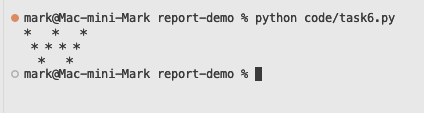
\includegraphics[width=0.65\linewidth]{task6-demo.png}
\end{vvsu_figure}

% Подглава - Задание 7
\subsection{Задание 7}

Задача заключалась в демонстрации работы основных арифметических и логических операторов языка Python.  
Для этого были созданы две переменные с произвольными числовыми значениями и проведены вычисления с использованием семи арифметических и шести операторов сравнения.  
На рисунке \ref{fig:code_task_7} представлен код программы.

\begin{vvsu_figure}{Листинг программы для задания 7}{fig:code_task_7}
  \begin{minipage}{.75\textwidth}
    \lstinputlisting[language=Python,basicstyle=\fontsize{10}{10}\linespread{1}\selectfont\ttfamily]{code/task7.py}
  \end{minipage}
\end{vvsu_figure}

Пояснение работы программы:
\begin{vvsu_list}
  \item Переменным x и y присвоены значения 10 и 3.
  \item В коде последовательно выполняются операции сложения, вычитания, умножения, деления, целочисленного деления, нахождения остатка и возведения в степень.
  \item Затем производится сравнение двух чисел по различным условиям (равенство, неравенство, больше, меньше и т.д.).
  \item Каждая операция сопровождается пояснительным текстом в выводе.
\end{vvsu_list}

После выполнения программы в консоли выводятся результаты всех арифметических и логических операций между переменными.

% Подглава - Задание 8
\subsection{Задание 8}

В этом задании необходимо было вывести строку, содержащую имя и возраст пользователя, с использованием f-строки.  
Такой способ форматирования позволяет удобно вставлять значения переменных непосредственно внутрь строки.  
На рисунке \ref{fig:code_task_8} представлен код программы.

\begin{vvsu_figure}{Листинг программы для задания 8}{fig:code_task_8}
  \begin{minipage}{.75\textwidth}
    \lstinputlisting[language=Python,basicstyle=\fontsize{10}{10}\linespread{1}\selectfont\ttfamily]{code/task8.py}
  \end{minipage}
\end{vvsu_figure}

Пояснение работы программы:
\begin{vvsu_list}
  \item Созданы две переменные: name -- содержит имя, и age -- возраст.
  \item Для объединения текста и значений переменных используется f-строка.
  \item F-строка позволяет вставлять значения переменных в нужные места строки без явной конкатенации.
\end{vvsu_list}

После выполнения программы в консоли отображается сообщение вида:  
<<Меня зовут Марк, мне 24 лет>>.

% Подглава - Задание 9
\subsection{Задание 9}

В этом задании нужно было собрать исходное предложение из нескольких переменных, каждая из которых хранит часть текста.  
Для объединения строк использовалась операция конкатенации при помощи знака +.  
На рисунке \ref{fig:code_task_9} представлен код программы.

\begin{vvsu_figure}{Листинг программы для задания 9}{fig:code_task_9}
  \begin{minipage}{.75\textwidth}
    \lstinputlisting[language=Python,basicstyle=\fontsize{10}{10}\linespread{1}\selectfont\ttfamily]{code/task9.py}
  \end{minipage}
\end{vvsu_figure}

Пояснение работы программы:
\begin{vvsu_list}
  \item Каждая из четырёх переменных (part1, part2, part3, part4) содержит\linebreak часть предложения.
  \item При помощи операции + и добавления пробелов создаётся итоговая строка.
  \item Полученная строка сохраняется в переменной sentence и выводится на экран.
\end{vvsu_list}

Результатом выполнения программы является восстановленное предложение:
<<Съешь ещё этих мягких французских булок, да выпей чаю>>.

% Подглава - Задание 10
\subsection{Задание 10}

В данном задании необходимо было создать строку <<Нет! Да!>>, повторяющуюся четыре раза подряд.  
Для решения использовалась операция умножения строк, позволяющая повторить заданную последовательность символов нужное количество раз.  
На рисунке \ref{fig:code_task_10} представлен код программы.

\begin{vvsu_figure}{Листинг программы для задания 10}{fig:code_task_10}
  \begin{minipage}{.75\textwidth}
    \lstinputlisting[language=Python,basicstyle=\fontsize{10}{10}\linespread{1}\selectfont\ttfamily]{code/task10.py}
  \end{minipage}
\end{vvsu_figure}

Пояснение работы программы:
\begin{vvsu_list}
  \item В переменной phrase хранится исходная строка <<Нет! Да!>>.
  \item С помощью операции умножения $phrase * 4$ строка повторяется четыре раза подряд.
  \item Результат сохраняется в переменной result и выводится в консоль.
\end{vvsu_list}

После выполнения программы в консоли отображается результат:  
<<Нет! Да!Нет! Да!Нет! Да!Нет! Да!>>.

% Подглава - Задание 11
\subsection{Задание 11}

В этом задании требовалось запросить у пользователя три числа, разделённые запятыми, а затем вычислить выражение (a + c) // b с использованием целочисленного деления.  
Результат необходимо вывести в консоль в виде поясняющего сообщения.  
На рисунке \ref{fig:code_task_11} представлен код программы.

\begin{vvsu_figure}{Листинг программы для задания 11}{fig:code_task_11}
  \begin{minipage}{.75\textwidth}
    \lstinputlisting[language=Python,basicstyle=\fontsize{10}{10}\linespread{1}\selectfont\ttfamily]{code/task11.py}
  \end{minipage}
\end{vvsu_figure}

Пояснение работы программы:
\begin{vvsu_list}
  \item Пользователь вводит три числа, разделённые запятыми, которые считываются функцией input().
  \item С помощью split(",") введённая строка разбивается на три элемента.
  \item Функция map(float, ...) преобразует каждое значение в тип с плавающей точкой.
  \item После этого вычисляется результат целочисленного деления суммы первого и третьего чисел на второе.
  \item Итоговый результат выводится на экран с помощью форматированной строки.
\end{vvsu_list}

После выполнения программа запрашивает ввод данных и выводит строку вида:  
<<Результат вычисления: 15>>.

% Подглава - Задание 12
\subsection{Задание 12}

В последнем задании лабораторной работы необходимо было запросить у пользователя слово, содержащее не менее десяти символов, и при помощи срезов вывести отдельные части строки, а также её обратный вариант.  
На рисунке \ref{fig:code_task_12} представлен код программы.

\begin{vvsu_figure}{Листинг программы для задания 12}{fig:code_task_12}
  \begin{minipage}{.75\textwidth}
    \lstinputlisting[language=Python,basicstyle=\fontsize{10}{10}\linespread{1}\selectfont\ttfamily]{code/task12.py}
  \end{minipage}
\end{vvsu_figure}

Пояснение работы программы:
\begin{vvsu_list}
  \item Программа запрашивает у пользователя ввод слова длиной не менее\linebreak десяти символов.
  \item Срез word[:4] возвращает первые четыре символа строки.
  \item Срез word[-2:] возвращает последние два символа.
  \item Срез word[3:8] выводит символы с четвёртого по восьмой.
  \item Срез word[::-1] переворачивает строку, выводя её в обратном порядке.
\end{vvsu_list}

После выполнения программа последовательно отображает результаты всех операций со срезами для введённого слова.


% \begin{application}{Приложение А}{Приложение А\\ \vspace{1em} Описание процесса работы с драйверами}
%   Самое обычное тестовое приложение
% \end{application}

\end{document}